% SIMILAR ISMIR PAPERS
% https://archives.ismir.net/ismir2023/paper/000045.pdf (I'm modeling my paper mostly from this)
% https://tomcollinsresearch.net/pdf/ismirReviewExamples.pdf (these are examples of ISMIR papers that aren't necessarily similar but have been heavily commented on by actual ISMIR reciewers)

% -----------------------------------------------
% Template for ISMIR Papers
% 2023 version, based on previous ISMIR templates

% Requirements :
% * 6+n page length maximum
% * 10MB maximum file size
% * Copyright note must appear in the bottom left corner of first page
% * Clearer statement about citing own work in anonymized submission
% (see conference website for additional details)
% -----------------------------------------------

\documentclass{article}
\usepackage[T1]{fontenc} % add special characters (e.g., umlaute)
\usepackage[utf8]{inputenc} % set utf-8 as default input encoding
\usepackage{ismir,amsmath,cite,url}
\usepackage{graphicx}
\usepackage{color}
\usepackage{listings}
\usepackage{float}

% Configure listings
\lstset{
    basicstyle=\footnotesize\ttfamily, % Set the font size and type
    breaklines=true,                    % Allow breaking lines
    tabsize=2,                          % Set tab size
    columns=flexible,                   % For better handling within columns
}

\usepackage{lineno}
\linenumbers

% Title. Please use IEEE-compliant title case when specifying the title here,
% as it has implications for the copyright notice
% ------
\title{Synthesizing Flexible, Composite Hierarchical Structure from Music Datasets}

% Note: Please do NOT use \thanks or a \footnote in any of the author markup

% Single address
% To use with only one author or several with the same address
% ---------------
\oneauthor
	{Ilana Shapiro}
	{UC San Diego \\ {\tt ilshapiro@ucsd.edu}}
 %{Names should be omitted for double-blind reviewing}
 %{Affiliations should be omitted for double-blind reviewing}

% Two addresses
% --------------
%\twoauthors
%  {First author} {School \\ Department}
%  {Second author} {Company \\ Address}

% Three addresses
% --------------\input{ISMIR2021_paper.tex}

%\threeauthors
%  {Ilana Shapiro} {Affiliation1 \\ {\tt author1@ismir.edu}}
%  {Second Author} {\bf Retain these fake authors in\\\bf submission to preserve the formatting}
%  {Third Author} {Affiliation3 \\ {\tt author3@ismir.edu}}

% Four or more addresses
% OR alternative format for large number of co-authors
% ------------
%\multauthor
%{First author$^1$ \hspace{1cm} Second author$^1$ \hspace{1cm} Third author$^2$} { \bfseries{Fourth author$^3$ \hspace{1cm} Fifth author$^2$ \hspace{1cm} Sixth author$^1$}\\
%  $^1$ Department of Computer Science, University , Country\\
%$^2$ International Laboratories, City, Country\\
%$^3$  Company, Address\\
%{\tt\small CorrespondenceAuthor@ismir.edu, PossibleOtherAuthor@ismir.edu}
%}

% For the author list in the Creative Common license, please enter author names. 
% Please abbreviate the first names of authors and add 'and' between the second to last and last authors.
\def\authorname{Ilana Shapiro}

% Optional: To use hyperref, uncomment the following.
%\usepackage[bookmarks=false,pdfauthor={\authorname},pdfsubject={\papersubject},hidelinks]{hyperref}
% Mind the bookmarks=false option; bookmarks are incompatible with ismir.sty.

\sloppy % please retain sloppy command for improved formatting

\begin{document}

%
\maketitle
%

%We adopt a ``(6+n)-page policy'' for ISMIR \conferenceyear. That is, each paper may have a maximum of six pages of technical content (including figures and tables) \textcolor{red}{with additional optional pages that contain only references and acknowledgments. Note that acknowledgments should not be included in the anonymized submission.}
%Paper should be submitted as PDFs and the \textcolor{red}{file size is limited to 10MB}. Please compress images and figures as necessary before submitting.

\begin{abstract}
Music is an innately hierarchical system, comprising multiple semantic levels informed by music theory. Such levels include formal structure segmentation, disjoint motif repetition, and harmonic and melodic contour. Historically, researchers in the music information retrieval community have focused on developing analyses for single levels in this hierarchy. However, existing research has addressed neither (1) how to combine arbitrarily many levels of structure analyses into a single unified model and (2) how to extract a representative such structure from a corpus of music, rather than just a single piece. In this work, we propose a novel data structure called the \textit{semantic temporal graph} that captures the semantic (i.e. hierarchical music theoretic) relationships between levels of the hierarchy, as well as the temporal relationships between adjacent-level analyses. Furthermore, given a corpus of such graphs derived from individual pieces, we introduce a method rooted in stochastic optimization to derive a representative $centroid$ graph encoding the music dataset's overall structure. We provide a qualitative evaluation of the semantic temporal graph [where we.....], as well as a quantitative evaluation of the centroid graph [where we...].
% and evaluate??
\end{abstract}


%
\section{Introduction}\label{sec:intro}
Music is both composed and comprehended with a hierarchical structure. Individual notes constitute the bottom of the hierarchy, followed by harmony, rhythmic patterns, motives, phrases, and finally large scale sections. Together, this composite hierarchy defines the overall structure of a piece \cite{msaf}.

Automatic identification of musical structure, also known as \textit{music structure analysis} (MSA), continues to be a major interest to both musicologists and the MIR community. Research thus far has focused on the automatic contiguous segmentation (both flat and hierarchical) of musical form \cite{msaf, checkerboard, sf, vmo_segmentation, cnmf, 2dfmc, eval_hier, olda, scluster, musicaiz, repetition_grammars_ismir2023, buisson_2022, cmu_dannenberg_2020}, which involves a boundary detection step followed by a segment labeling step, as well as motif detection \cite{Hsiao_2023_motifs, vmo_motifs, features_motifs}, which looks for disjoint repeating musical patterns. More recently, researchers have also developed avenues for harmonic \cite{chen_2019_harmony}, functional harmonic \cite{chen_2018_harmony}, and melodic \cite{salamon_2013_melody, kosta_22_melody, midibert} contour extraction. The techniques used are diverse, ranging from matrix factorization to deep learning in both supervised and unsupervised settings. All of these tasks have been proposed in annual competitions of the Music Information Retrieval eXchange (MIREX) \cite{MIREX_2017_form, MIREX_2017_motif, MIREX_2010_harmony, MIREX_2021_melody}, which provides a standard format for their outputs. 

To our knowledge, all existing MSA research addresses a single aspect of the compositional hierarchy, such as motif extraction, or melodic contour. There is currently no notion of how reconcile differing levels of the hierarchy into a single, unified model of  structure, even though their amalgamation is central to a piece's compositional architecture and cohesive integrity. Indeed, Dai et al. have demonstrated empirically that the levels' contents are not formed in isolation, revealing significant interactions different structural levels \cite{cmu_dannenberg_2020}. In identifying the critical components necessary for integrating the hierarchical levels, we find that there are two central challenges: how to convey each level's semantic, music theoretic level in the hierarchy, and how to encapsulate the temporal relationships between the results of structural analyses at adjacent hierarchical levels. 

Furthermore, prior MSA research has only addressed the problem of identifying structure in a single piece, and there is presently no methodology for describing the overall structure of a musical corpus, even across existing single-level analyses. The one exception is Oriol Nieto's proposed technique for merging multiple segment boundary annotations \cite{msaf}, but this is intended to be used with multiple boundary detection algorithms over a single piece to alleviate the problem of subjectivity, and does not address the problem of reconciling differing labels.  

\subsection{Contributions}\label{subsec:contributions}

To address the first gap, in Section \ref{sec:representation}, we develop the notion of a \textit{semantic temporal graph} (STG), a $k$-partite directed acyclic graph (DAG) where the semantic, music theoretic levels of the compositional hierarchy are represented as levels in the $k$-partite structure, nodes represent structure labels that are the results of the relevant analysis at each level, and edges between nodes of adjacent levels convey the temporal relationships between those structure labels. Each node has an associated time interval determined by the relevant MSA algorithm. A node must have one or two parents at the level above it: one if its associated time interval is a total subset of its parents, and two if its time interval begins in one parent and ends in the other. In order to easily parse the results of MSA algorithms into this data structure, the standard MIREX format is adhered to.

Importantly, the STG is incredibly flexible, and supports the representation of arbitrarily many layers and layer types. Furthermore, the STG is totally decoupled from any specific MSA algorithm or input format, meaning that the chosen MSA algorithm for any level can be easily swapped out, as long as its output adheres to the standard MIREX format. This is crucial as single-level MSA algorithms are constantly improving, and the STG must be adaptable enough to accommodate this.

Finally, to address the second gap, in Section \ref{sec:synthesis} we examine the problem of finding a \textit{centroid}, or most representative, graph given a corpus of the k-partite semantic temporal DAGs derived from individual pieces. We use the label-aware graph edit distance as the similarity metric between two graphs. Given such a set of graphs $G$, we seek to construct the STG $g*$ that minimizes this distance from $g*$ to every graph in $G$. This is a constraint satisfaction problem, but one that is intractable to solve deterministically. Thus, we must rely on approximation techniques, and utilize Markov Chain Monte Carlo methods, demonstrating how to use the Metropolis Hastings algorithm to infer an optimal solution and thus arrive at the centroid graph most descriptive of the entire corpus by construction.\footnote{Source code for this project can be found at https://github.com/ilanashapiro/constraints\_project}

\section{Related work}\label{sec:related_work}
The majority of existing MSA algorithms focus on the contiguous formal segmentation task: boundary detection, followed by section labeling. Segmentation algorithms can be flat or hierarchical (where each level is an increasingly granular contiguous segmentation of the piece). Existing approaches generally utilize matrix factorization, formal grammars, or more recently, neural networks. Oriol Nieto's Music Structure Analysis Framework (MSAF) toolkit \cite{msaf} features most of the state-of-the art matrix factorization approaches for audio, including ordinal linear discriminant analysis \cite{olda}, convex nonnegative matrix factorization \cite{cnmf}, checkerboard \cite{checkerboard}, spectral clustering \cite{scluster}, the Structural Features algorithm \cite{sf}, 2D-Fourier Magnitude Coefficients \cite{2dfmc}, and the Variable Markov Oracle \cite{vmo_segmentation}. These methods use variants of self-similarity matrices (SSMs) for boundary detection, which are symmetric matrices storing pair-wise comparisons between a given set of features. To assign labels, various methods including Gaussian mixture models and nearest neighbor search are employed \cite{msaf}. 

More recently, both supervised \cite{wang_2021} and unsupervised \cite{mccallum_2021, buisson_2022} deep learning approaches to segmentation have studied, as have graph- and grammar-based approaches. Hernandez-Olivan et al. use the graph-based G-PELT algorithm \cite{musicaiz}, while Dai et al. employ a graph-based approach informed by interactions between sections, melody, harmony and rhythm \cite{cmu_dannenberg_2020}. In the grammar realm, Finkensiep et al. attempt a unified model of structure by using a minimal context-free grammar to combine repetition with formal prototypes in a tree-based approach, but they still only operate within the contiguous segmentation domain \cite{repetition_grammars_ismir2023}. 

In the motif extraction domain, algorithms search for disjoint, repeating, and possibly overlapping patterns in a piece. They generally fall into three categories: string-based approaches (e.g. the Variable Markov Oracle \cite{vmo_motifs}), where music data is represented as a one-dimensional pitch sequence and repeated patterns are detected with sub-string matching; geometry-based approaches (e.g. Hsiao et al's BPS-motif discovery algorithm \cite{Hsiao_2023_motifs}), where music data is represented as multidimensional point sets and \textit{translatable subsets} identify repeating patterns; and feature-based (e.g. \cite{features_motifs}) approaches, which learn features from music data, and retrieve patterns with clustering or classification of the features as repeated patterns.
%The Variable Markov Oracle offers a quality string-based approach \cite{vmo_motifs}, although our experiments reveal that it struggles to detect motifs of length $>2$.  

Recent approaches in harmony identification are centered around neural networks, such as using multi-task
learning with recurrent neural networks and long short term memory units to detect functional harmonic relationships in a piece \cite{chen_2018_harmony}, as well as developing transformer models to improve chord recognition through incorporating chord segmentation into the recognition process \cite{chen_2019_harmony}. Until very recently, Justin Salamon's Melodia algorithm was the state of the art in melody extraction. It comprises sinusoid extraction, salience functions, contour creation, and melody selection, and automatically estimates the fundamental frequency corresponding to the pitch of the predominant melodic line of a piece of polyphonic music. Since then, approaches have shifted to neural networks, such as lightweight deep bidirectional
LSTM models \cite{kosta_22_melody} and transformers \cite{midibert}.

To our knowledge, little work has been done in developing a unified model of structure for either a single piece or across a corpus. The closest we are aware of is Halley Young's \textit{prototype graph}, a bipartite graph that represents musical form as a network of relationships between ``prototype nodes" (specific musical elements) and the music they represent, as well as the music-theoretic relationships between musical spans and their respective nodes \cite{young_2022}. However, the prototype graph does not encode hierarchy, and it is limited to a single piece.


\section{Abstract Representation}\label{sec:representation}


\subsection{Semantic Temporal Graph} \label{subsec:st_graph}
We seek a unified model of musical structure that captures semantic, music theoretic levels of the compositional hierarchy, as well as the temporal relationships between them. The \textit{semantic temporal graph}, or STG, is a novel data structure serving as a meta-representation of musical structure that unifies these objectives. The STG is $k$-partite directed acyclic graph (DAG). Each of the $k$ layers encodes a level in the semantic hierarchy dictated by music theory. From top to bottom, the music theoretic hierarchy is formed by large scale form, motifs, rhythmic patterns, harmony, and finally melodies constituting specific note events with a certain timbre quality, duration, and pitch \cite{msaf}. Individual levels themselves can form sub-hierarchies of increasing granularity, as is commonly seen with the segmentation algorithms corresponding to large scale sections.

In the STG, nodes encode labels from the relevant MSA algorithm. Each node also has an associated time interval given by the algorithm. At each level, these intervals are converted to indices by ordering their start times. Edges encode temporal relationships between nodes of adjacent levels. Specifically, for node $n$ at level $i$, $n$ must have either one or two parents in level $i-1$: one if its associated time interval is a total subset of its parent's, and two if its time interval begins in one parent's, and ends in the other's.

\subsection{Building the Graph}\label{subsec:build}

In order to visualize the STG more clearly, we must first establish how it is built. In this paper, we build STGs that unify hierarchical formal segmentation and disjoint motif repetition, with plans in the near future to add layers for rhythm, harmony, and melody. In order to parse the results of any MSA algorithm into a format suitable for the STG, we must first consider the standard MIREX formats they adhere to. 

The structural segmentation task was most recently proposed in the 2017 MIREX competition \cite{MIREX_2017_form}. It defines the following standard output format:
\begin{lstlisting}
<onset_time(sec)>\t<offset_time(sec)>\t<label>\n
<onset_time(sec)>\t<offset_time(sec)>\t<label>\n
...
\end{lstlisting}
where $\backslash$t denotes a tab and $\backslash$n denotes the end of line. The $<$ and $>$ characters are not included. Thus, an example output file could look like:
\begin{lstlisting}
0.000    5.223    A
5.223    15.101   B
15.101   20.334   A
\end{lstlisting}
Hierarchical segmentations will have multiple of these lists separated by a newline.

MIREX 2017 also dictates the standard output format for motif detection algorithms \cite{MIREX_2017_motif}. Ontimes (in seconds) of notes in the pattern in the left-hand column, with their MIDI note numbers on the right. Each occurrence of a discovered pattern is given before moving on to the next pattern, and occurrences do not have to be of the same length. An example output would resemble:
\begin{lstlisting}
pattern1 
occurrence1 
7.00000, 45.00000 
... 
11.00000, 60.00000 
occurrence2 
31.00000, 57.00000 
...
patternM 
occurrence1 
9.00000, 58.00000 
...
occurrencem 
100.00000, 62.00000 
...
\end{lstlisting}

Given these standard MIREX formats, we must parse this data into a format suitable for the STG. Each ``chunk" of the data, separated by a newline, forms a level in the STG, and each line in a chunk corresponds to a node. Consider Figure \ref{fig:form_parse}, which demonstrates the parsing process for a segmentation hierarchy with two levels. We start with the MIREX segmentation output in step 1. In step 2, we number each segmentation level (i.e. text chunk) and extract the segment label and time interval from each line. This gives us the preliminary node label \textbf{S}\{segment label\}\textbf{L}\{segment level number\}\textbf{I}\{time interval\}. Finally, in step 3, we transform each time interval into an index representing that line's position in the level, sorted by interval start time. In the case of segmentation, this matches the line order in the MIREX output. We now have the final segmentation node label \textbf{S}\{segment label\}\textbf{L}\{segment level number\}\textbf{N}\{label index within level\}. 

\begin{figure}[h!]
  \centering
  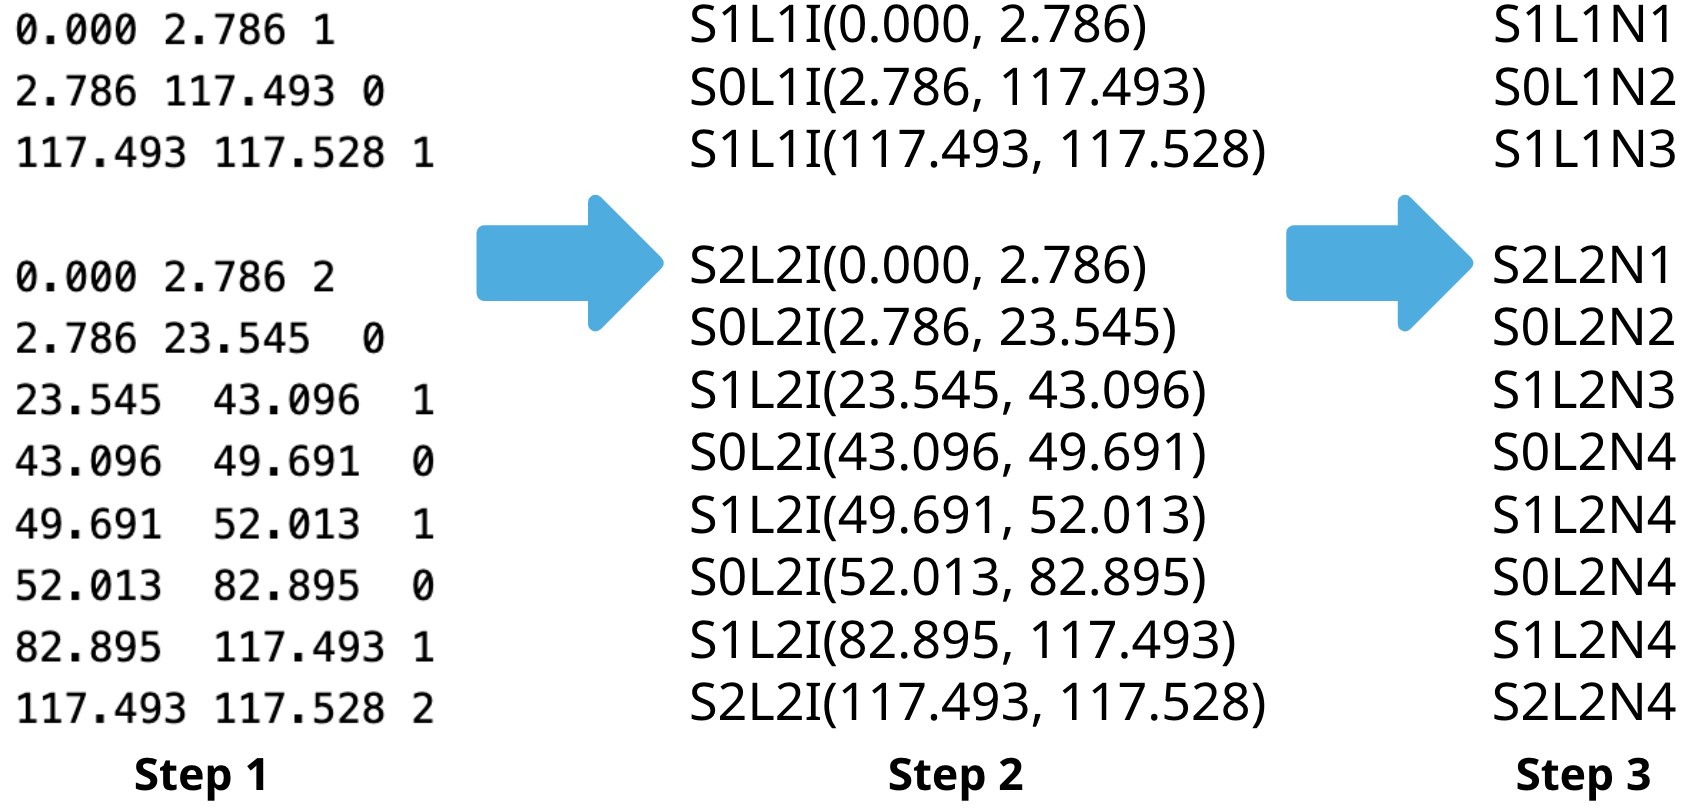
\includegraphics[width=\linewidth]{figs/form_parse}
  \caption{Parsing Formal Segmentation}
  \label{fig:form_parse}
\end{figure}

We repeat this process for motifs as in Figure \ref{fig:motif_parse}. Motif analyses are single level, i.e. they do not output sub-hierarchies like segmentation can do. Consider the MIREX motif output in step 1. Each pattern (i.e. motif) occurrence's time interval is defined as the ontime of its first note to its last, and we extract pattern and occurrence numbers in step 2 to arrive at the preliminary node label \textbf{P}\{pattern number\}\textbf{O}\{occurrence number\}\textbf{I}\{time interval\}. We then order the preliminary labels by start time, as unlike in segmentation, pattern occurrences are not ordered chronologically in MIREX format. We then assign indices to this ordering to arrive at the final motif node label \textbf{P}\{pattern number\}\textbf{O}\{occurrence number\}\textbf{N}\{chronologic occurrence index\}. This is reflected in step 3, where occurrence 2 of pattern 1 is assigned index 3 instead of 2. 

\begin{figure}[h!]
  \centering
  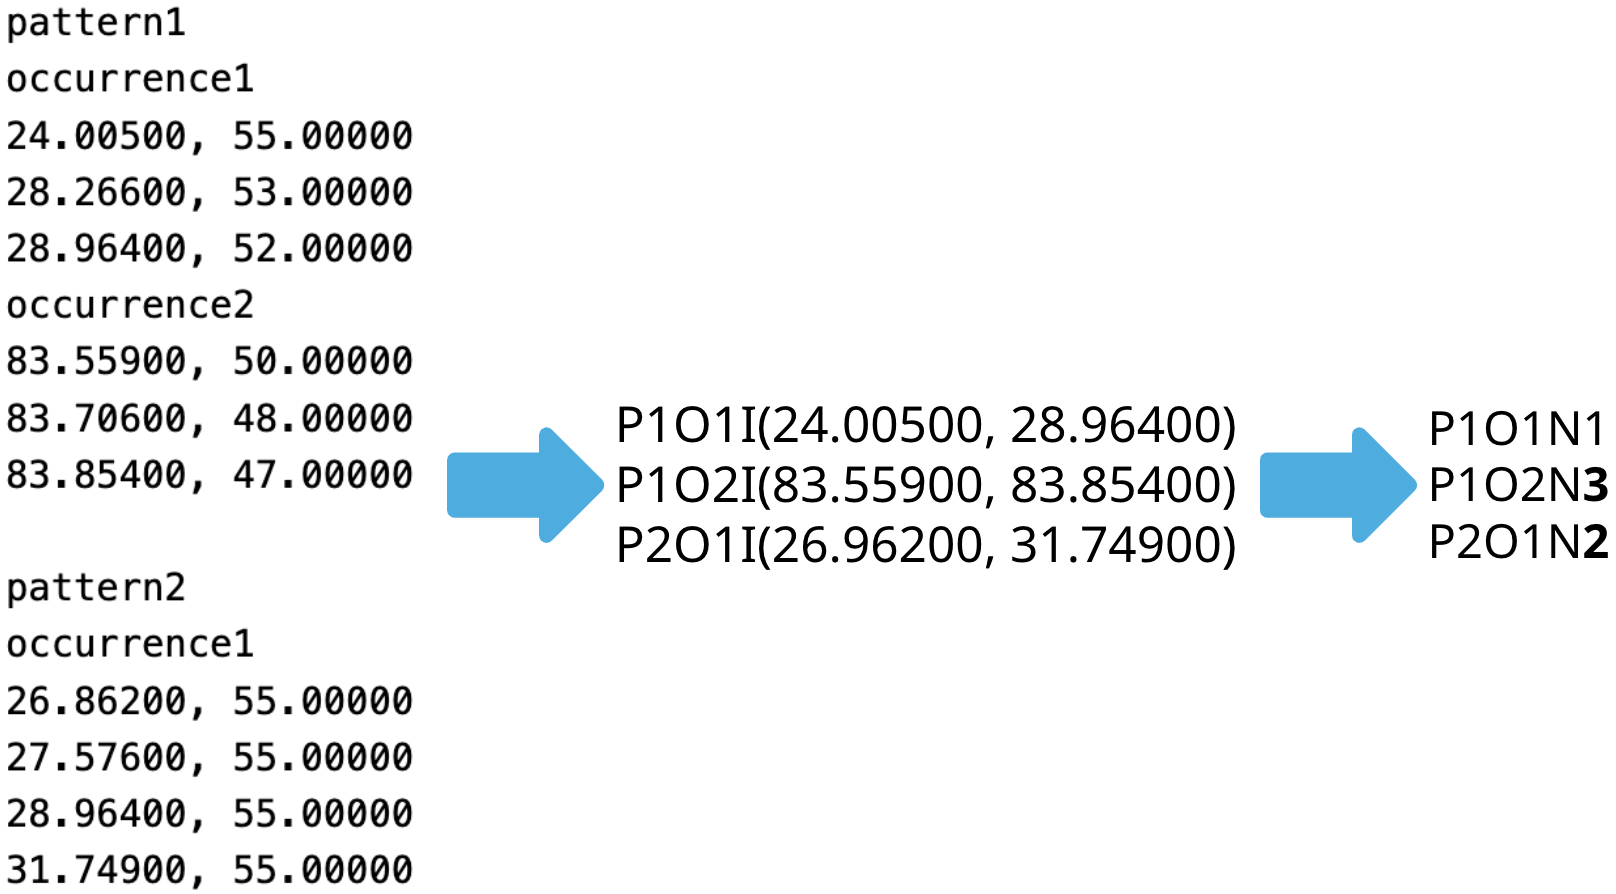
\includegraphics[width=\linewidth]{figs/motif_parse}
  \caption{Parsing Motifs}
  \label{fig:motif_parse}
\end{figure}

In all cases, the time interval is stored as node metadata, and determines what that node's parent(s) will be.

\subsection{STG Examples}\label{subsec:stg_ex}

In the following examples, we use hierarchical spectral clustering from the MSAF toolkit for segmentation \cite{msaf, scluster}, and Hsiao et al's BPS-motif discovery algorithm for motifs \cite{Hsiao_2023_motifs}. To better visualize the STG's structure, first consider the following subgraph taken from an STG generated for the first movement exposition of the piano transcription of Beethoven's Symphony No. 1, Op. 21 in Figure \ref{fig:stg_ex}.\footnote{MIDI file is from the LOP database, which can be found here: https://qsdfo.github.io/LOP/database} The nodes are taken from levels 4 and 5 of the segmentation sub-hierarchy.
\begin{figure}[h!]
  \centering
  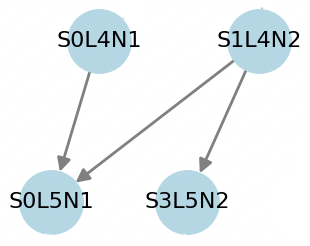
\includegraphics[width=0.45\linewidth]{figs/stg_example}
  \caption{STG Subgraph Example}
  \label{fig:stg_ex}
\end{figure}
Node S3L5N2’s time interval is a total subset of S1L4N2's, while S0L5N1’s time interval starts in S0L4N1’s, but ends in S2L4N2’s. The entire STG generated for this piece, unifying hierarchical formal segmentation with disjoint motif detection, is shown in Figure \ref{fig:stg_full}. The segmentation nodes are easily visible, and the motif nodes form the crowded bottom layer.

\begin{figure}[h!]
  \centering
  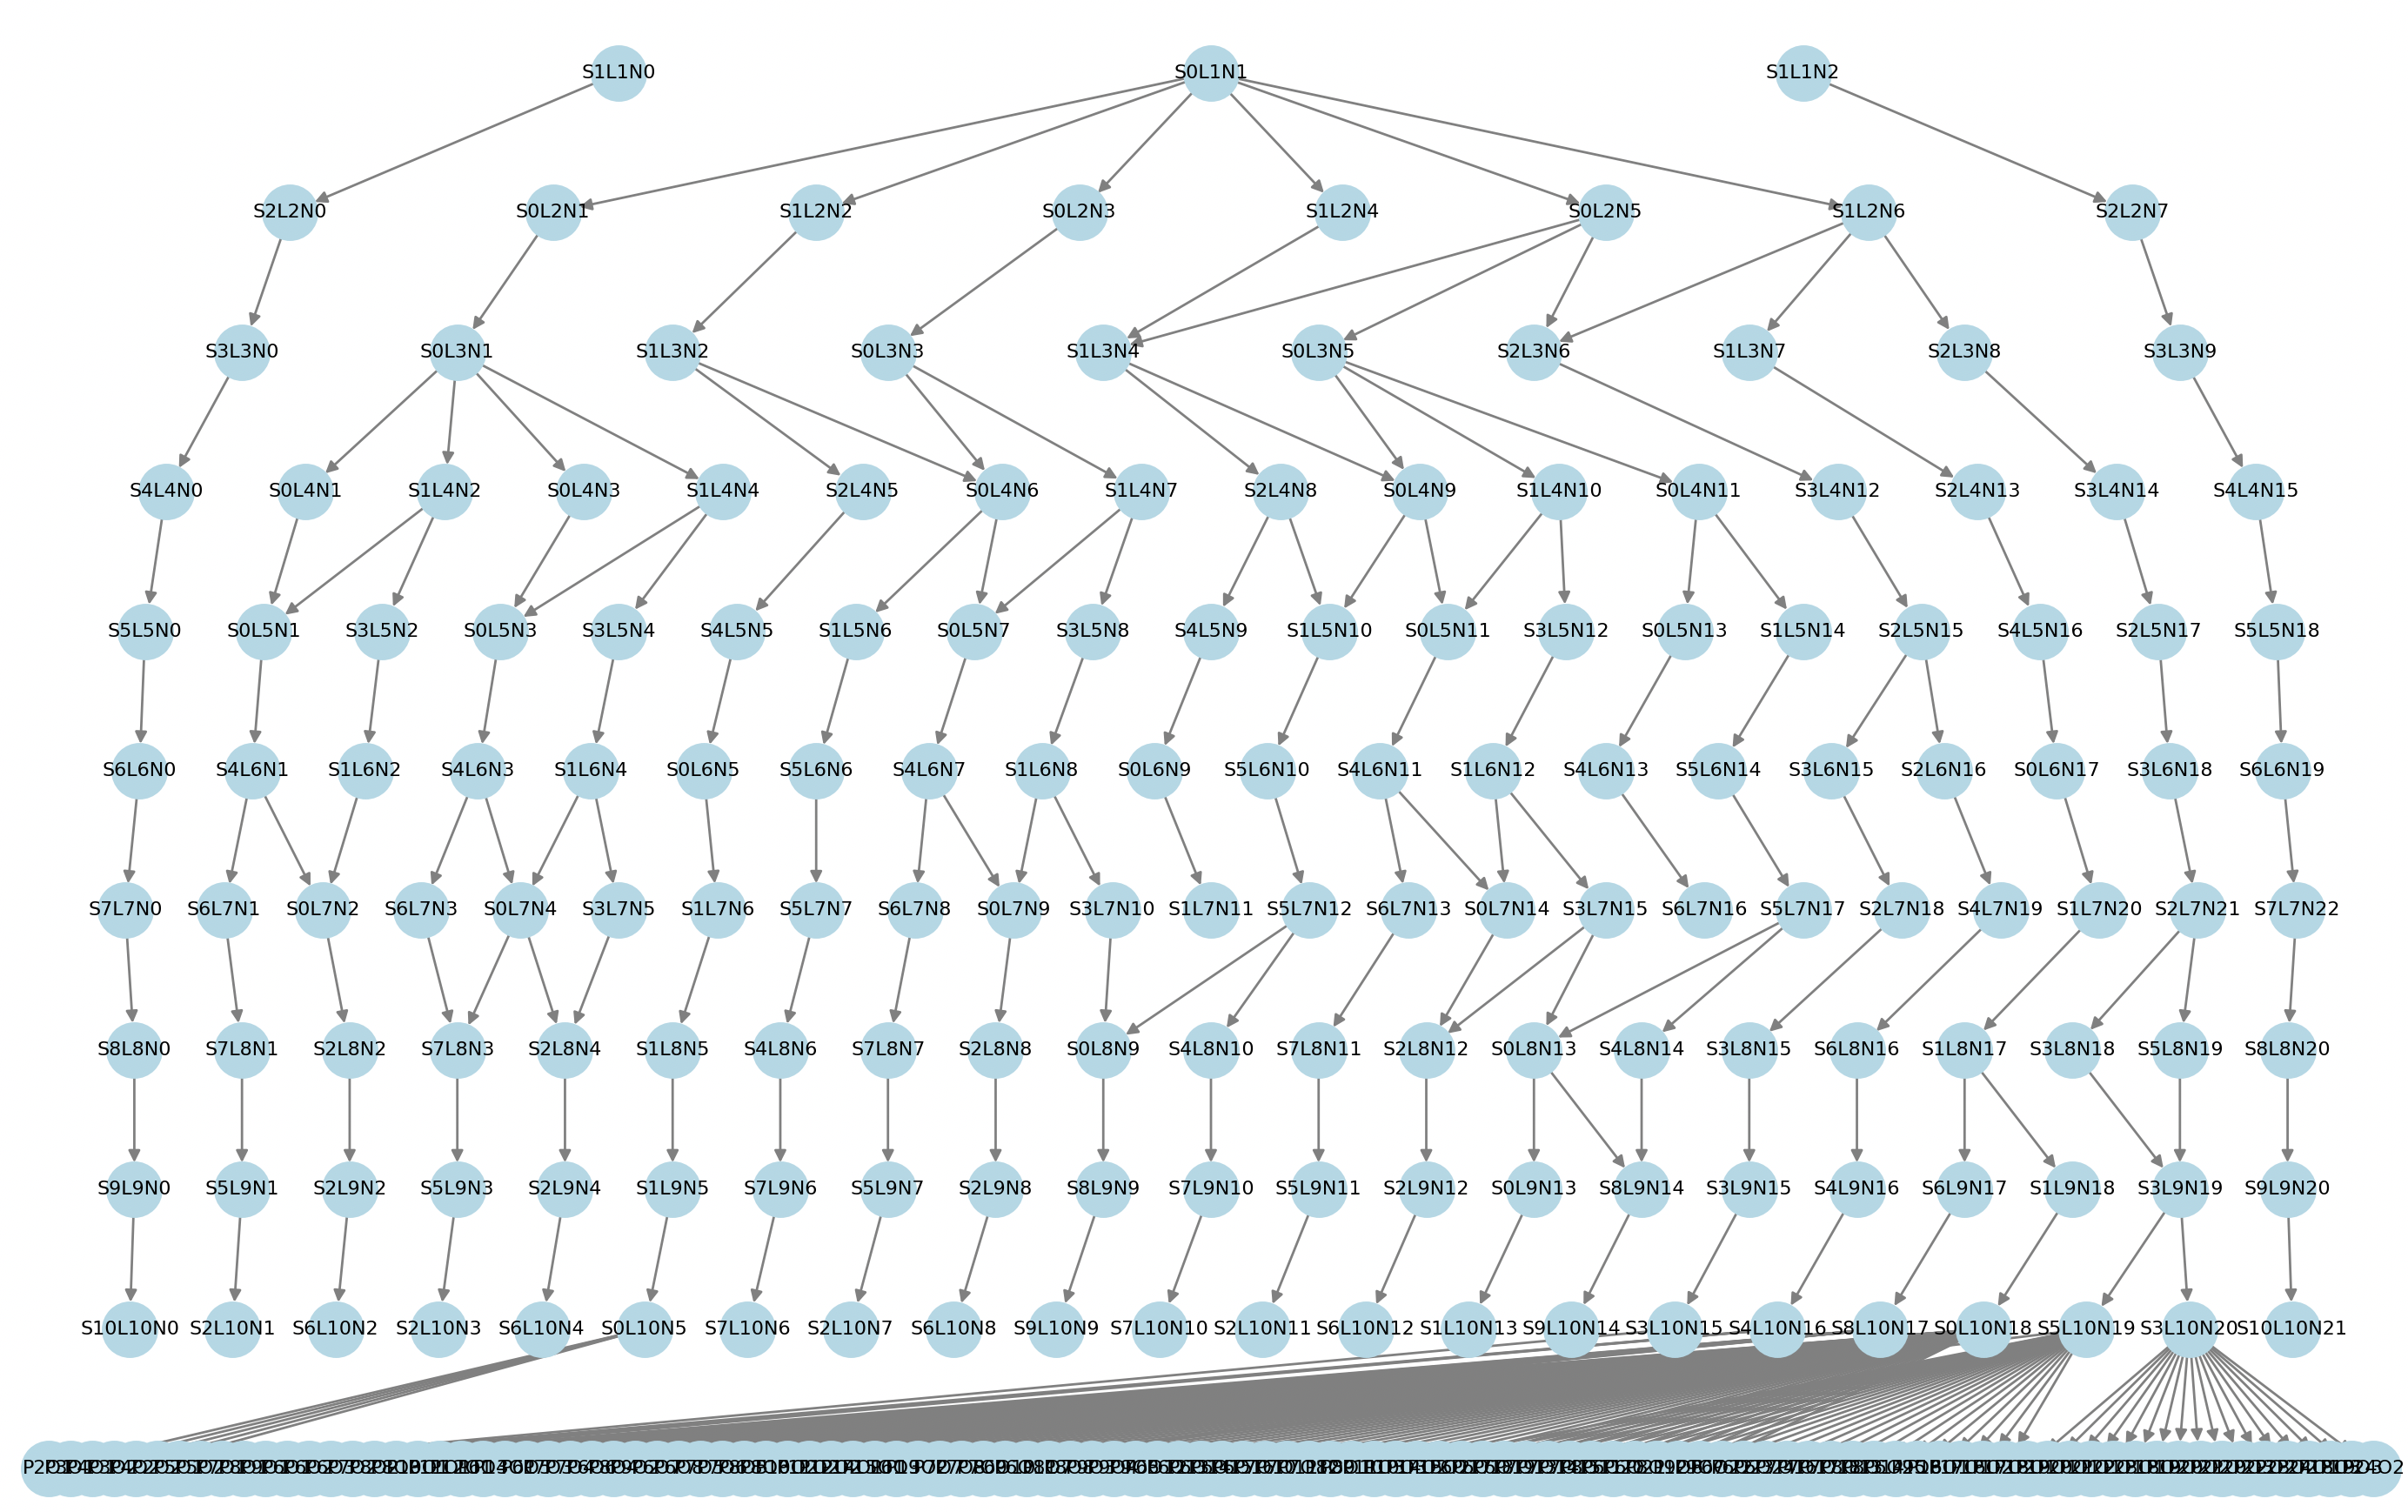
\includegraphics[width=\linewidth]{figs/stg_full}
  \caption{STG Subgraph Example}
  \label{fig:stg_full}
\end{figure}

\section{Synthesis}\label{sec:synthesis}
\subsection{Distance Metric}\label{subsec:dist_metric}
\subsection{Stochastic Optimization}\label{subsec:stoch_opt}

%\section{Evaluation} \label{subsec:eval}

\section{Conclusions and Future Work}
In this paper we have presented a unified meta-representation of complete musical structure that encapsulates the both the intrinsic compositional hierarchy Such a model is essential to comprehending the fundamental system that underlies the core architecture of the piece

not only the composition and structure of the piece but also its perception and existence within the musical domain.

To our knowledge, all existing MSA research addresses a single aspect of the compositional hierarchy, such as motif extraction, or melodic contour. There is currently no notion of how reconcile differing levels of the hierarchy into a single, unified model of structure, even though their amalgamation is central to a piece's compositional architecture and cohesive integrity.


Since repetition structure is an aspect of human music cognition, the overarching objective of our approach is to approach human listening.

%\section{Acknowledgments}
%\textbf{Do not include in your submission, only in your camera ready version}. This section can be used to refer to any individuals or organizations that should be acknowledged in this paper. This section does \textit{not} count towards the page limit for scientific content.


% bib sources list:
% https://archives.ismir.net/ismir2023/paper/000045.pdf (new ISMIR paper on hierarchical grammars)
% https://archives.ismir.net/ismir2014/paper/000226.pdf (previous work on grammar extraction for form)
% https://archives.ismir.net/ismir2019/paper/000039.pdf (grammar for Harmony -- didn't include in bib)
% https://citeseerx.ist.psu.edu/document?repid=rep1&type=pdf&doi=a602b8d972f68b100350c5dc54681cc44f31493a (sCluster)
% https://www.ee.columbia.edu/~dpwe/pubs/McFeeE14-segments.pdf (OLDA)
% https://www.frontiersin.org/journals/psychology/articles/10.3389/fpsyg.2017.01337/full (evaluating hierarchical analyses)
% https://ccrma.stanford.edu/~urinieto/MARL/publications/Nieto-Dissertation.pdf (MSAF)
% https://ccrma.stanford.edu/~urinieto/MARL/publications/NietoBello-ICASSP14.pdf (2D-FMC)
% https://cacm.acm.org/research/stochastic-program-optimization/ (stochastic program optimization)
% https://escholarship.org/uc/item/7tg5c8rb / https://www.semanticscholar.org/paper/Structural-segmentation-with-the-Variable-Markov-Wang-Mysore/1f9ac4bb9527d47deec00f24efd72d7c1796ca0c / https://www.ismir2015.uma.es/articles/78_Paper.pdf(VMO)
% https://ismir2023program.ismir.net/poster_145.html (motif extraction)
% https://proceedings.neurips.cc/paper_files/paper/2022/hash/f13ceb1b94145aad0e54186373cc86d7-Abstract-Conference.html (halley, prototype graph)
% https://arxiv.org/pdf/2209.07974.pdf / https://www.sciencedirect.com/science/article/pii/S2352711023000614 (musicaiz)
% https://hal.science/hal-03278537/ (morpheauS)
% https://ismir2018.ircam.fr/doc/pdfs/178_Paper.pdf (harmony 1)
% https://archives.ismir.net/ismir2019/paper/000030.pdf (harmony 2)
% https://arxiv.org/pdf/2107.05223.pdf (melody 1)
% https://archives.ismir.net/ismir2022/paper/000091.pdf (melody 2)
% https://www.justinsalamon.com/uploads/4/3/9/4/4394963/jsalamon_phdthesis.pdf (melody 3)



\bibliography{ISMIRtemplate}

% For non bibtex users:
%\begin{thebibliography}{citations}
% \bibitem{Author:17}
% E.~Author and B.~Authour, ``The title of the conference paper,'' in {\em Proc.
% of the Int. Society for Music Information Retrieval Conf.}, (Suzhou, China),
% pp.~111--117, 2017.
%
% \bibitem{Someone:10}
% A.~Someone, B.~Someone, and C.~Someone, ``The title of the journal paper,''
%  {\em Journal of New Music Research}, vol.~A, pp.~111--222, September 2010.
%
% \bibitem{Person:20}
% O.~Person, {\em Title of the Book}.
% \newblock Montr\'{e}al, Canada: McGill-Queen's University Press, 2021.
%
% \bibitem{Person:09}
% F.~Person and S.~Person, ``Title of a chapter this book,'' in {\em A Book
% Containing Delightful Chapters} (A.~G. Editor, ed.), pp.~58--102, Tokyo,
% Japan: The Publisher, 2009.
%
%
%\end{thebibliography}

\end{document}

